\documentclass[twoside, 11pt]{exam}

\usepackage[T1]{fontenc}
\usepackage[utf8]{inputenc}
\usepackage[dutch]{babel}

\usepackage[font={small,sf},labelfont={bf},labelsep=endash]{caption}
\usepackage{fouriernc}
\usepackage[detect-all, binary-units, separate-uncertainty=true,
            per-mode=symbol, retain-explicit-plus, range-phrase={ tot },
            list-final-separator={ en }, output-decimal-marker={,}]
            {siunitx}

\usepackage{setspace}
\setstretch{1.2}

\setlength{\parskip}{\smallskipamount}
\setlength{\parindent}{0pt}

\usepackage{geometry}
\geometry{a4paper, vmargin=3cm, inner=3cm, outer=2cm, head=14pt}

\usepackage{float}

\usepackage[fleqn]{amsmath}
\numberwithin{equation}{section}
\numberwithin{figure}{section}

\usepackage{graphicx}
\graphicspath{{Figures/}}
\usepackage{subfig}

\usepackage[svgnames]{xcolor}
\usepackage{tikz}
\usepackage{tikz-3dplot}
\usepackage{pgfplots}
\usetikzlibrary{plotmarks,circuits.ee.IEC,pgfplots.groupplots,external,calc}
\pgfplotsset{compat=1.3}

\usepackage{minted}
\usepackage{amsthm}
\usepackage{relsize}
\usepackage{xspace}
\usepackage{url}
\usepackage{sansmath}
\usepackage{titling}


\theoremstyle{plain}
\newtheorem*{note}{Note}


\newcommand{\figref}[1]{Figuur~\ref{#1}}

\newcommand{\hisparc}{\textsmaller{HiSPARC}\xspace}
\newcommand{\kascade}{\textsmaller{KASCADE}\xspace}
\newcommand{\sapphire}{\textsmaller{SAPPHiRE}\xspace}
\newcommand{\jsparc}{\textsmaller{jSparc}\xspace}
\newcommand{\hdf}{\textsmaller{HDF5}\xspace}
\newcommand{\aires}{\textsmaller{AIRES}\xspace}
\newcommand{\csv}{\textsmaller{CSV}\xspace}
\newcommand{\python}{\textsmaller{PYTHON}\xspace}
\newcommand{\corsika}{\textsmaller{CORSIKA}\xspace}
\newcommand{\labview}{\textsmaller{LabVIEW}\xspace}
\newcommand{\dspmon}{\textsmaller{DSPMon}\xspace}
\newcommand{\daq}{\textsmaller{DAQ}\xspace}
\newcommand{\adc}{\textsmaller{ADC}\xspace}
\newcommand{\adcs}{\textsmaller{ADC}s\xspace}
\newcommand{\Adcs}{A\textsmaller{DC}s\xspace}
\newcommand{\hi}{\textsc{h i}\xspace}
\newcommand{\hii}{\textsc{h ii}\xspace}
\newcommand{\mip}{\textsmaller{MIP}\xspace}
\newcommand{\hisparcii}{\textsmaller{HiSPARC II}\xspace}
\newcommand{\hisparciii}{\textsmaller{HiSPARC III}\xspace}
\newcommand{\pmt}{\textsmaller{PMT}\xspace}
\newcommand{\pmts}{\textsmaller{PMT}s\xspace}
\newcommand{\gps}{\textsmaller{GPS}\xspace}

\DeclareSIUnit{\electronvolt}{\ensuremath{\mathrm{e\!\!\:V}}}

\DeclareSIUnit{\unitsigma}{\ensuremath{\sigma}}
\DeclareSIUnit{\mip}{\textsmaller{MIP}}
\DeclareSIUnit{\adc}{\textsmaller{ADC}}

\DeclareSIUnit{\gauss}{G}
\DeclareSIUnit{\parsec}{pc}
\DeclareSIUnit{\year}{yr}


%% Document style definitions

% macros and commands
\newcommand{\shorttitle}[1]{\def\theshorttitle{#1}}
\newcommand{\docindex}[1]{\def\thedocindex{#1}}
\newcommand{\version}[1]{\def\theversion{#1}}
\newcommand{\setsectionstyle}[2]{
  \colorlet{seccolor}{#1}
  \def\thesectiontitle{#2}
}

\newcommand{\setdocumentstyle}[4]{
  \setsectionstyle{#1}{#2}
  \docindex{#3}
  \shorttitle{#4}
}

% document types
\newcommand{\docalgemeen}[2]{\setdocumentstyle{red}{Algemeen}{#1}{#2}}
\newcommand{\docinstallatie}[2]{\setdocumentstyle{Gold}{Detector installatie}{#1}{#2}}
\newcommand{\docdetector}[2]{\setdocumentstyle{blue}{Detector}{#1}{#2}}
\newcommand{\docweerstation}[2]{\setdocumentstyle{LightSlateGray}{Weerstation}{#1}{#2}}
\newcommand{\docbliksem}[2]{\setdocumentstyle{orange}{Bliksem}{#1}{#2}}
\newcommand{\docanalyse}[2]{\setdocumentstyle{DarkViolet}{Data analyse}{#1}{#2}}
\newcommand{\docwerkblad}[2]{\setdocumentstyle{ForestGreen}{Werkbladen}{#1}{#2}}
\newcommand{\docdocent}[2]{\setdocumentstyle{DarkKhaki}{Uitwerkingen}{#1}{#2}}
\newcommand{\docopdrachten}[2]{\setdocumentstyle{Silver}{Opdrachten}{#1}{#2}}
\newcommand{\docrecept}[2]{\setdocumentstyle{Navy}{Recept}{#1}{#2}}

\pgfmathsetlengthmacro\stylemarginsep{+1cm}
\pgfmathsetlengthmacro\stylethumbsep{+.75cm}

\newcommand{\rightthumb}{
\begin{tikzpicture}[remember picture, overlay]
  % vertical line
  \draw[seccolor]
    ($(current page.north east) + (-\stylemarginsep, -.5cm)$) --
    ($(current page.south east) + (-\stylemarginsep, .5cm)$);

  % thumb
  \fill[seccolor]
    ($(current page.north east) +
      (-\stylemarginsep, -2cm -\thedocindex * \stylethumbsep)$)
      rectangle +(.5cm, -.5cm);
\end{tikzpicture}
}

\newcommand{\leftthumb}{
\begin{tikzpicture}[remember picture, overlay]
  % vertical line
  \draw[seccolor]
    ($(current page.north west) + (\stylemarginsep, -.5cm)$) --
    ($(current page.south west) + (\stylemarginsep, .5cm)$);

  % thumb
  \fill[seccolor]
    ($(current page.north west) +
      (\stylemarginsep, -2cm -\thedocindex * \stylethumbsep)$)
      rectangle +(-.5cm, -.5cm);
\end{tikzpicture}
}

\renewcommand{\maketitle}{
  \suppressfloats

  \begin{titlepage}
  \thispagestyle{\defaultstyle}
  \let\endtitlepage\relax
  \begin{tikzpicture}[remember picture, overlay,
    titlebox/.append style={seccolor, fill, text=white, minimum height=1cm,
      font=\sffamily\huge, draw=none},
    authorbox/.append style={minimum height=.5cm, font=\sffamily}]

    \node[titlebox, anchor=north west, shift={(3cm, -1cm)}] at
      (current page.north west) {\thesectiontitle};

    \node[anchor=north west, shift={(2.83cm, -2cm)}] at
      (current page.north west) {
\includegraphics[scale=.8]{../HiSPARC_header}};

    \node[titlebox, anchor=north east, shift={(-\stylemarginsep, -1cm)}] at
      (current page.north east) {\thetitle};

    \node[authorbox, anchor=north east, shift={(-\stylemarginsep, -2cm)}] at
      (current page.north east) {\theauthor};
  \end{tikzpicture}
  \end{titlepage}
}


\newcommand{\defaultstyle}{headandfoot}

% style definitions
\pagestyle{\defaultstyle}
\chead{\oddeven{\rightthumb}{\leftthumb}}
\cfoot{\theshorttitle\ -- \thepage}
\lfoot{\oddeven{}{\textcolor{gray}{\smaller Versie \theversion}}}
\rfoot{\oddeven{\textcolor{gray}{\smaller Versie \theversion}}{}}

\renewcommand{\thequestion}{\textbf{Opdracht \arabic{question}:}}
\renewcommand{\solutiontitle}{\noindent\textbf{Antwoord:}\enspace}
\newcommand{\makelines}[1]{\ifprintanswers\else\fillwithlines{#1\linefillheight}\fi}

\ifdefined\showanswers
  \printanswers
\else
  \noprintanswers
\fi


\usepackage{hepnames}
\usepackage{mhchem}

\DeclareRobustCommand{\PgDpp}{\HepParticle{\Delta}{}{++}\xspace}

\title{Opdrachten: Elementaire deeltjes}
\author{C.G.N. van Veen}
\docwerkblad{5}{ED}
\version{1.0}

\begin{document}

\maketitle

\begin{questions}

\uplevel{\section{Hadronen}}

\question
Elementaire deeltjes worden onderverdeeld in quarks en leptonen.
\begin{parts}
\part Noem twee eigenschappen die quarks en leptonen met elkaar gemeen hebben.
\makelines{2}
\begin{solution}
    Ze hebben beide spin \textonehalf. Ze zijn beide elementair,
    d.w.z. niet verder deelbaar.
\end{solution}
\part Noem twee eigenschappen waarin quarks en leptonen van elkaar verschillen.
\makelines{2}
\begin{solution}
    Quarks vormen samen hadronen. Leptonen hebben geen `kleur'.
    Quarks hebben een fractionele lading.
\end{solution}
\end{parts}

\question
Wanneer twee quarks combineren, dan richten de spins zich `parallel'
of `tegengesteld'.
\begin{parts}
\part Beredeneer dat de quarks in een pion met tegengestelde spin zijn gecombineerd.
\makelines{2}
\begin{solution}
    Pionen zijn mesonen en bestaan dus uit twee quarks. Elk
    quark heeft een spin + of - \textonehalf. Combinaties van twee spins
    kunnen dus opleveren spin +1, -1 of 0. Het pion heeft een spin van
    0. Dus in het pion moeten de quarks spin -\textonehalf \xspace en
    +\textonehalf \xspace hebben.
\end{solution}
\part Beredeneer de manier waarop de 3 quarks in een neutron hun spins hebben gericht.
\makelines{2}
\begin{solution}
    Een neutron is opgebouwd uit 3 quarks. Als we de spins bij
    elkaar optellen, kan dat dus opleveren -1\textonehalf,
    -\textonehalf\xspace en +\textonehalf \xspace  +1\textonehalf.
\end{solution}
\end{parts}

\question
Samengestelde deeltjes (``hadronen'') worden onderverdeeld in mesonen en baryonen.
\begin{parts}
\part In welk opzicht zijn mesonen anders van samenstelling dan baryonen? Leg uit.
\makelines{2}
\begin{solution}
    Mesonen bestaan uit twee quarks en hadronen bestaan uit drie
    quarks.
\end{solution}
\part Komen er in de natuur mesonen voor met een massa groter dan die van een baryon?
Zo ja, welke.
\makelines{2}
\begin{solution}
    Ja, bijvoorbeeld het \PD meson heeft een grotere rustmassa
    dan het neutron of het proton.
\end{solution}
\part Komen er in de natuur mesonen voor met een negatieve lading?
\makelines{2}
\begin{solution}
    Ja, bijvoorbeeld \Ppiminus-meson.
\end{solution}
\end{parts}

\question
Alle deeltjes hebben een anti-deeltje.
\begin{parts}
\part Welke deeltjes uit BINAS-26 zijn identiek aan hun eigen antideeltje?
\makelines{2}
\begin{solution}
    Fotonen, \Ppizero en het majorana-deeltje.
\end{solution}
\part Noem drie redenen waarom het proton niet het antideeltje van het \Ppiplus-meson kan zijn.
\makelines{2}
\begin{solution}
    Een proton bestaat uit drie quarks, het \Ppiplus uit twee.
    Het proton en het \Ppiplus hebben beide een + lading.
    Het proton is een baryon en heeft daardoor een halftallige spin, een meson
    heeft een heeltallige spin.
\end{solution}
\end{parts}

\question
Een \PKplus -deeltje bestaat uit een \Pup -quark (`up') en een \APqs-quark
(`anti-strange'), schematisch weergegeven als \PKplus = [\Pup\APqs].
\begin{parts}
\part Is het \PKplus -deeltje een meson of een baryon?
\makelines{2}
\begin{solution}
    Het \PKplus bestaat uit twee quarks en is dus een meson.
\end{solution}
\part Beredeneer hoe een \PKm-deeltje moet zijn opgebouwd.
\makelines{2}
\begin{solution}
    Uit een \APup -quark (`anti-up') en een \Pqs-quark. Door het antideeltje te
    nemen van de aanwezige quarks is de lading van het \PKm-deeltje dus
    negatief geworden.
\end{solution}
\end{parts}

\question
Het \Ppiplus-meson bestaat uit de quarks \Pup en \APdown  (`up' en `anti-down')
en is positief geladen.
\begin{parts}
\part Bereken dat de lading van een \Ppiplus-meson gelijk is aan +1e.
\makelines{2}
\begin{solution}
    Het up-quark heeft lading $\frac{2}{3}$  en de lading van het down quark
    is -$\frac{1}{3}$, de lading van het antidown quark (\Paqd) is
    +$\frac{1}{3}$. De lading van het \Ppiplus is dus: $\frac{2}{3}$ +
    $\frac{1}{3}$ = 1.
\end{solution}
\part Leg uit dat een \PSigmaplus-deeltje niet een quarkcombinatie [\Pstrange\Pdown\Pdown]
kan zijn.
\makelines{2}
\begin{solution}
    Als je de ladingen van deze quarks optelt krijg je -1.
    Het \PSigmaplus deeltje heeft lading +1.
\end{solution}
\end{parts}

\question
Een proton bestaat uit de combinatie [\Pup\Pup\Pdown].
\begin{parts}
\part Noteer de quarksamenstelling van het antideeltje van een proton.
\makelines{2}
\begin{solution}
    \APup,\APup en \APdown of \Pap = [\APup\APup\APdown]
\end{solution}
\part Bereken de lading van het antiproton.
\makelines{2}
\begin{solution}
    -$\frac{2}{3}$ - $\frac{2}{3}$ + $\frac{1}{3}$ = -1.
\end{solution}
\end{parts}

\question
Een neutron bestaat uit de combinatie [\Pup\Pdown\Pdown].
\begin{parts}
\part Bereken de lading van een antineutron.
\makelines{2}
\begin{solution}
    Een anti neutron bestaat dus uit [\APup\APdown\APdown].
    Hieruit volgt: -$\frac{2}{3}$ + $\frac{1}{3}$ + $\frac{1}{3}$ = 0.
\end{solution}
\uplevel{De gegeven quark-combinatie is niet stabiel.}
\part Welke drie deeltjes ontstaan bij het verval van een neutron?
\makelines{2}
\begin{solution}
    $\Pn \rightarrow \Pp + \Pe + \Pagne$.
    Een neutron vervalt in een proton, een elektron en een anti-elektronneutrino.
\end{solution}
\end{parts}


\uplevel{\section{Reacties}}

\question
Op de schets van een bellenvatfoto is te zien, dat bij de botsing van een
aanstormend pion op een proton, een kaon en een lambda ontstaan. Zie
\figref{fig:bellenvat}.
Zowel het kaon als het lambda zijn instabiel.
Zoek met BINAS uit wat de identiteit is van deeltje x en van deeltje y.
\makelines{2}
\begin{solution}
    Deeltje x = \Ppiplus en deeltje y = \Pp.  Want \PKzero vervalt door
    een \Ppiplus en een \Ppiminus uit te zenden. \PLambda vervalt door een
    \Ppiminus en een \Pp uit te zenden (te verklaren door behoud van
    Baryon getal en behoud van lading).
\end{solution}
\begin{figure}[h]
    \centering
    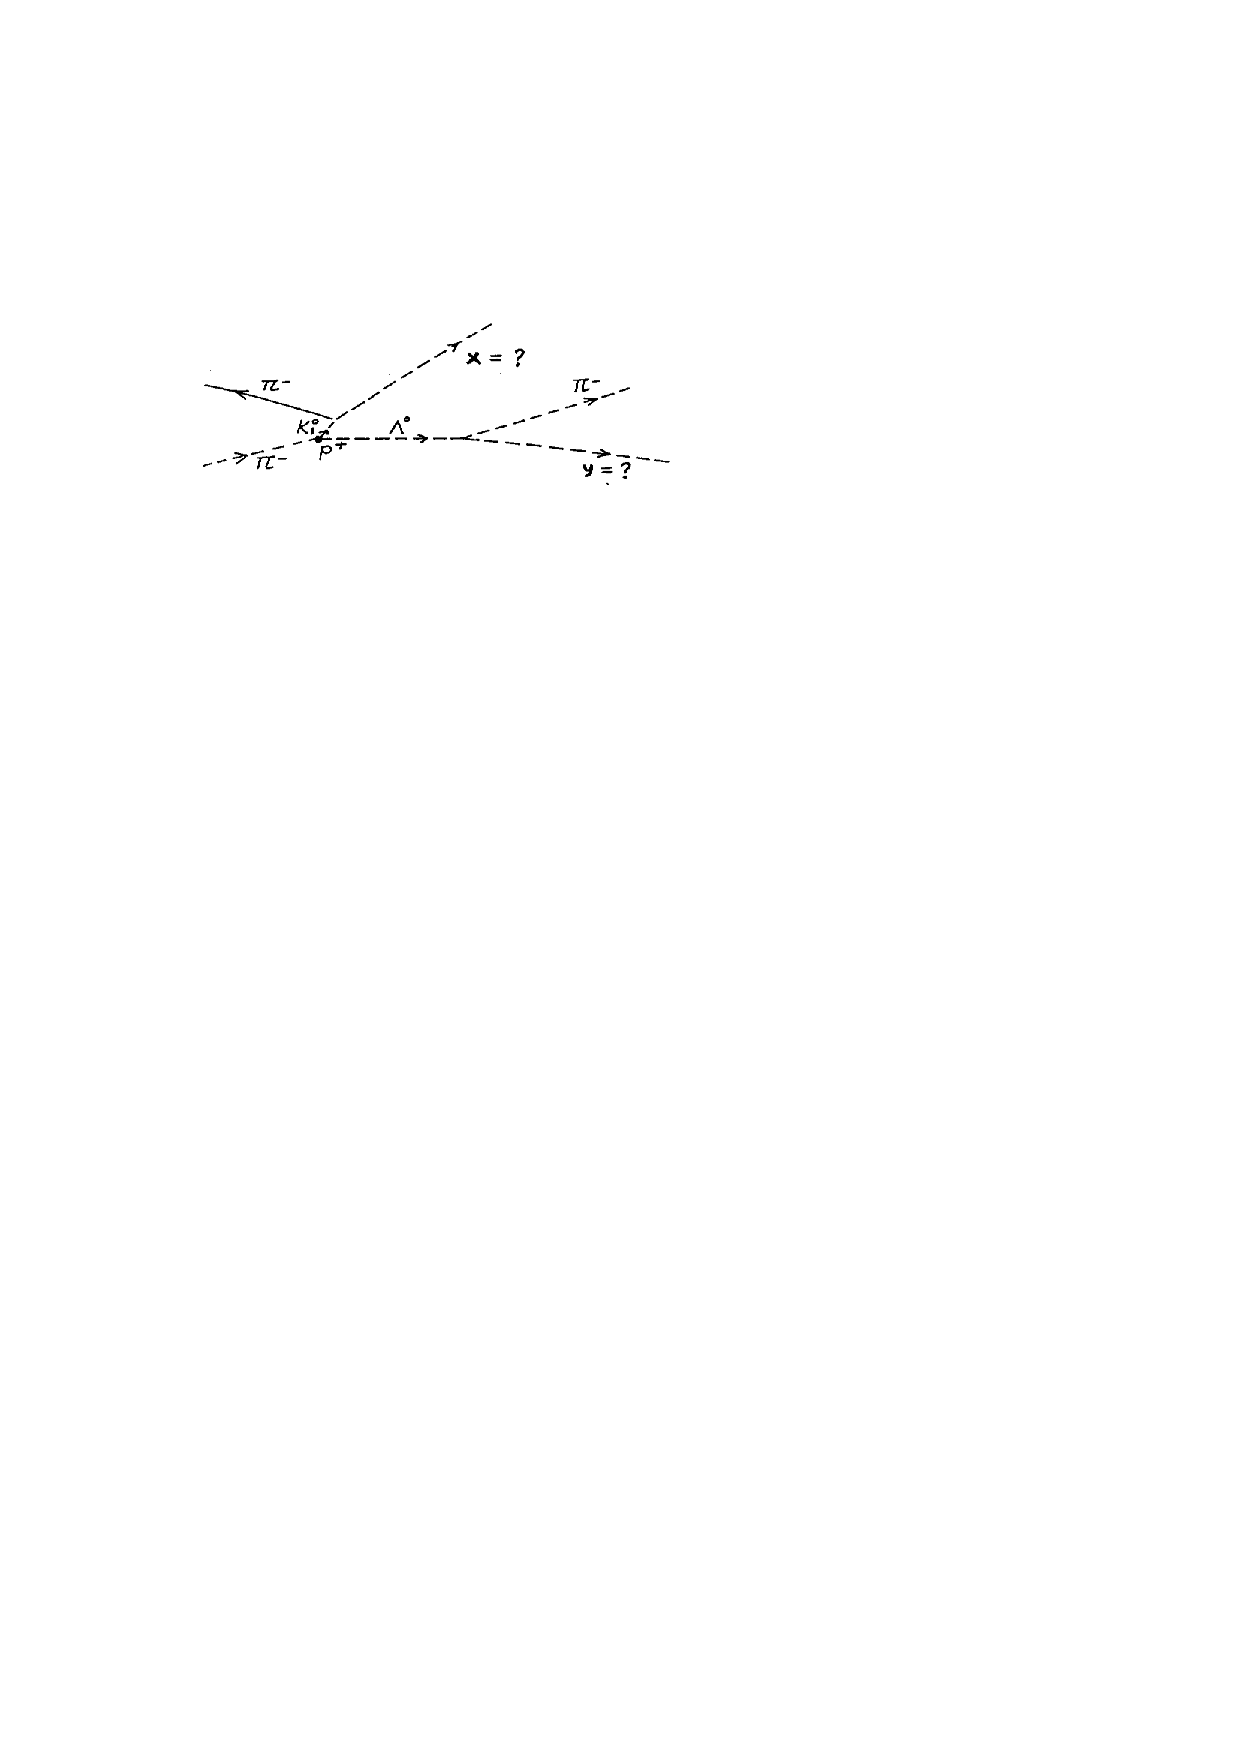
\includegraphics{bellenvat}
    \caption{Bellenvat schets van een foto van de reacties van een pion.}
    \label{fig:bellenvat}
\end{figure}


\question
In BINAS-26 wordt als eenheid van massa vermeld: \si{MeV.c^{-2}}.
\begin{parts}
\part Wat wordt hiermee bedoeld?
\makelines{2}
\begin{solution}
    \begin{eqnarray*}
        E = m \cdot c^2 \rightarrow m = \frac{E}{c^2} \\
        \left[m\right] = \left[ \si{MeV.c^{-2}} \right]
    \end{eqnarray*}
\end{solution}
\part Hoeveel keer zo traag is het muon vergeleken met het electron? Leg uit.
\makelines{2}
\begin{solution}
    Massa staat voor de traagheid van een deeltje. Dus:
    \begin{eqnarray*}
    m(\Pmu) = \SI{105,6}{\mega\electronvolt\per c\squared} \\
    m(\Pe) = \SI{0.51}{\mega\electronvolt\per c\squared} \\
    \text{aantal keer trager:} \quad \frac{105,6}{0,51} = \SI{2,1e2}{}
    \end{eqnarray*}
\end{solution}
\part Hoeveel energie is er minstens nodig om een muon en zijn antideeltje te
creëren? Leg uit.
\makelines{2}
\begin{solution}
    $2\times \SI{105,6}{\mega\electronvolt\per c\squared} = \SI{211}{\mega\electronvolt\per c\squared}$
\end{solution}
\end{parts}

\question
Het \Ppiplus-meson bestaat uit de quarks \Pup en \APdown.
\begin{parts}
\part Bereken het massadefect bij het combineren van een \Pup met een \APdown quark.
\emph{Binas geeft een indicatie van de quarkmassa! Quarks bestaan niet los!}
\makelines{2}
\begin{solution}
    \begin{eqnarray*}
     \Delta m = m(\Ppi) - m(\Pup + \APdown) = \SI{139.6}{\mega\electronvolt\per c\squared}
    - (\SI{2.0}{\mega\electronvolt\per c\squared} +
    \SI{4.8}{\mega\electronvolt\per c\squared}) \\= \SI{132.8}{\mega\electronvolt\per c\squared}
    \end{eqnarray*}
\end{solution}
\part Bereken de bindingsenergie van de quarks in het \Ppiplus-meson.
\makelines{2}
\begin{solution}
    Massadefect is dan gelijk aan de
    bindingsenergie. Er is een enorme bindingsenergie als quarks
    combineren tot elementaire deeltjes, vandaar dat we quarks nooit los
    aantreffen, maar altijd als combinaties in deeltjes.
\end{solution}
\end{parts}

\question
Gegeven: een reactie waarbij uit één baryon een nieuw baryon én een meson ontstaat:
\ce{{\PgDpp} -> \Pp+ + \Ppiplus}
\begin{parts}
\part Uit welke quarks bestaan het $\Pp^+$ en \Ppiplus?
\makelines{2}
\begin{solution}
    $\Pp^+ = [\Pup\Pdown\Pdown] \quad\text{en}\quad \Ppiplus = [\Pup\APdown]$
\end{solution}
\part Uit welke quarkcombinatie bestaat het \PgDpp-deeltje?
\makelines{2}
\begin{solution}
    Het \PgDpp bestaat uit $[\Pup\Pup\Pup]$
\end{solution}
\uplevel{De massa van het \PgDpp-deeltje is \SI{1230}{MeV.c^{-2}}.}
\part Bereken de massa van het \PgDpp-deeltje, uitgedrukt in kilogram.
\makelines{2}
\begin{solution}
    \begin{eqnarray*}
    \SI{938.49}{\mega\electronvolt\per c\squared}= 1 u = \SI{1.667e-27}{\kilo\gram} ; \\
    m(\PgDpp) = (1230/938,49)* \SI{1.667e-27}{\kilo\gram} = \SI{2.201e-27}{\kilo\gram}
    \end{eqnarray*}
\end{solution}
\part Hoeveel energie komt vrij bij het verval van het \PgDpp-deeltje?
Geef de berekening.
\makelines{3}
\begin{solution}
    \begin{eqnarray*}
    \PgDpp \rightarrow \Pp^+ + \Ppiplus \\
    m(\PgDpp) = \SI{1230}{\mega\electronvolt\per c\squared}  \\m(\Pp^+) = \SI{938}{\mega\electronvolt\per c\squared}; \\
    m(\Ppiplus) = \SI{139.6}{\mega\electronvolt\per c\squared} \\
    \Delta m = \SI{152.4}{\mega\electronvolt\per c\squared}
    \end{eqnarray*}
\end{solution}
\end{parts}


\uplevel{\section{De zon en neutrino's}}

\question
De energieproductie van een ster is voor een deel afkomstig van kernfusie
(het overige deel is het gevolg van gravitatiecontractie). Voor fusie is in
een ster een overvloed aan waterstofkernen aanwezig. Via een reeks van vier
opeenvolgende stappen wordt waterstof omgezet in helium. Bij de eerste stap
ontstaan onder andere een deuteriumkern en een neutrino:

%\ce{\Pp^+ + \Pp^+ -> ^2_1H + \Pnu + ? } \\
\begin{align}
\cee{ \label{eq:deuterium}
^1_1H+ + ^1_1H+ &-> ^2_1H+ + e^+ + \nu \\
?  + ^2_1H+  &-> ^3_2He^2+ + \gamma \\
^3_2He^2+ + ^3_2He^2+  &-> ^4_2He^2+ + 2\cdot {?} \\
e^+ + ? &-> \gamma  \\
}
\end{align}
De laatste stap betreft het ``opruimen'' van de positronen door middel van
annihilatie.
\begin{parts}
\part Wat is in de opeenvolgende stappen de identiteit van de met ``?'' aangegeven deeltjes?
\makelines{3}
\begin{solution}
    Stap 2: \cee{ ^1_1H+}.
    Stap 3: \cee{ ^1_1H+}.
    Stap 4: \Pelectron.
\end{solution}
\part Hoeveel waterstofkernen zijn (netto) nodig geweest om één heliumkern te vormen?
\makelines{2}
\begin{solution}
    Er zijn 4 waterstofkernen nodig.
\end{solution}
\part Geef de netto-vergelijking voor de productie van één heliumkern.
\makelines{3}
\begin{solution}
    Je moet stap 1 en stap 2 vermenigvuldigen met 2, om in stap 3
    de benodigde twee He-3 kernen te krijgen.
    \begin{align*}
    \cee{ \label{eq:nettofusion}
    4\cdot ^1_1H+ &-> ^4_2He + 2 \cdot e^+ + 2 \cdot \Pnue }
    \end{align*}
\end{solution}
\part Bereken de energie die bij de productie van één heliumatoom vrijkomt.
\makelines{3}
\begin{solution}
    We gebruiken de netto vergelijking bij vraag c. De positronen
    annihileren en produceren gamma's.

    \begin{align*}
    \cee{
     m( 4 \cdot ^1_1H+) &=  4 \cdot \SI{1.008}{\atomicmassunit} = \SI{4.032}{\atomicmassunit}\\
     m(^4_2He) &= \SI{4.0026}{\atomicmassunit} \\
     \Delta m &= \SI{0.029}{\atomicmassunit}\\
     E &= 0,0294 * 931,49 =  \SI{27.3}{\mega\electronvolt}
     }
    \end{align*}
\end{solution}
\end{parts}


\question
De energieproductie van onze zon vindt voornamelijk plaats in de kern doordat
waterstofkernen fuseren tot helium.
Bij één fusieproces wordt 26,731 \si{MeV} energie geproduceerd en komen
twee neutrino's vrij.
In \figref{fig:Zonsdoorsnede} zie je een gamma en een neutrino de zon
verlaten. Beide zijn ongeveer geproduceerd op hetzelfde moment.
\begin{figure}[h]
\centering
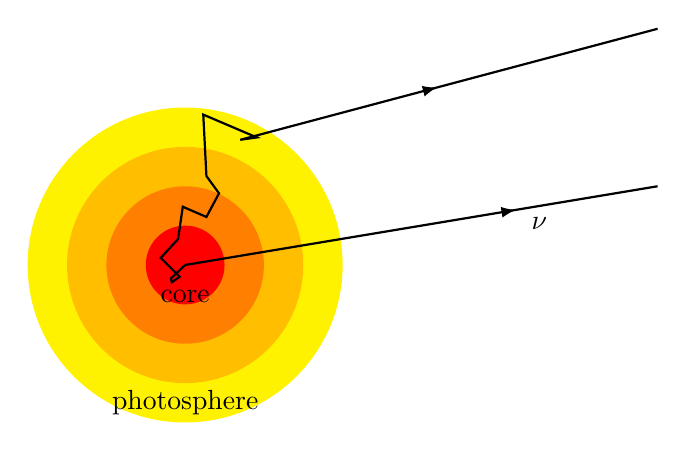
\begin{tikzpicture}[
  particle/.style={thick,decoration={markings, mark=at position .7 with {\arrow[>=latex]{>}}},postaction=decorate}
]
\fill[yellow] (0, 0) circle (2cm);
\fill[orange!50!yellow] (0, 0) circle (1.5cm);
\fill[orange] (0, 0) circle (1cm);
\fill[red] (0, 0) circle (.5cm);

\node at (0, -.4cm) {core};
\node at (0, -1.75cm) {photosphere};

\draw[particle] (0, 0) -- (6cm, 1cm) node[below,near end] {\Pneutrino};
\draw[particle] (0, 0)  -- (-0.18, -0.17)  -- (-0.17, -0.22)  -- (-0.07, -0.15)  -- (-0.31, 0.09)  -- (-0.09, 0.33)  -- (-0.03, 0.74)  -- (0.27, 0.61)  -- (0.43, 0.91)  -- (0.27, 1.13)  -- (0.23, 1.91)  -- (0.91, 1.62)  -- (0.70, 1.59) -- (6cm, 3cm) node[below,near end] {\Pphoton};
\end{tikzpicture}
\caption{Zonsdoorsnede}
\label{fig:Zonsdoorsnede}
\end{figure}
\begin{parts}
\part Leg uit dat het neutrino de zon veel sneller zal verlaten dan het gamma.
\makelines{2}
\begin{solution}
    Het neutrino heeft
    (bijna) geen interactie met materie dus zal met ongeveer de
    lichtsnelheid door de zon gaan. Het gammafoton wordt keer op keer geabsorbeerd en
    weer uitgezonden door atomen in de zon. Voordat het foton het zonsoppervlak heeft bereikt,
    kunnen er wel een miljoen jaar verstreken zijn.
\end{solution}
\part Zoek op in BINAS hoe groot het uitgestraald vermogen van de zon is.
\makelines{2}
\begin{solution}
    Het uitgestraalde vermogen is $P = \SI{0.390e27}{\watt}$.
\end{solution}
\part Bereken het aantal neutrino's dat de zon per seconde uitzendt.
\makelines{5}
\begin{solution}
    We weten het vermogen van de zon en wat er per reactie aan energie vrijkomt.
    Per (`netto'-) reactie komen er twee neutrino's vrij.
    \begin{eqnarray*}
    E_\text{reactie} = \SI{26.731}{\mega\electronvolt} \times\SI{1.602e-13}{\joule \per\mega\electronvolt} \\
    E_\text{reactie} = \SI{4.2823e-12}{\joule}\\
    n = \frac{P}{E} = \frac{\SI{0.390e27}{\watt}}{\SI{4.2823e-12}{\joule}}\\
    n = 2\times \num{9.11e37} = \num{1.82e38}
    \end{eqnarray*}
\end{solution}
\part Bereken de massavermindering van de zon in één jaar.
\makelines{4}
\begin{solution}
    Het aantal reacties per s is \num{9.11e37}. In één jaar zitten
    \SI{3.15e7}{\second}. Per reactie wordt $\frac{\SI{26.731}{\mega\electronvolt}}{\SI{938.49}{\mega\electronvolt\per\atomicmassunit} }$
    = \SI{0.0285}{\atomicmassunit} omgezet. Dit is \SI{4.748e-29}{\kilo\gram} per reactie.
    Dus aantal reacties per jaar:
    \begin{eqnarray*}
    n_\text{reacties} = \SI{3.15e7}{\second}\times\SI{9.11e37}{\per\second} \\
    n_\text{reacties} = \num{2.87e45} \\
    m_\text{omgezet in één jaar} = \num{2.87e45} \times \SI{4.748e-29}{\kilo\gram} = \SI{1.36e17}{\kilo\gram}
    \end{eqnarray*}
\end{solution}
\uplevel{Alle neutrino's verlaten de zon. Ze worden naar alle richtingen uitgezonden.
Op aarde is een neutrinodetector opgesteld met een naar de zon gekeerde
doorsnede van 5,0 m$^{2}$.}
\part Zoek op in BINAS hoe groot de afstand van de detector tot de zon gemiddeld
is.
\makelines{2}
\begin{solution}
    De afstand van de aarde tot de zon is (gem.) \SI{1.496e11}{\meter}
\end{solution}
\part Bereken hoeveel neutrino's per seconde de detector bereiken.
\makelines{4}
\begin{solution}
    De geproduceerde neutrino's worden verdeeld over een boloppervlak met een straal van \SI{1.496e11}{\meter}.
    Voor het oppervlak van een bol geldt: $A = 4 \pi r^{2}$.
    \begin{eqnarray*}
    A_\text{bol} = 4 \cdot \pi \cdot (\SI{1.496e11}{}) ^2\\
    A_\text{bol} = \SI{2.812e23}{\meter\squared}\\
    n_\text{neutrino's door detector} = \frac{5.0}{\SI{2.812e23}{}} * \SI{1.82e38}{}\\
    n_\text{neutrino's door detector} = \SI{3.2e15}{}
    \end{eqnarray*}
\end{solution}
\end{parts}

\end{questions}
\end{document}
